\documentclass[11pt,a4paper,draft=false]{report}
\usepackage{amsmath,amsthm,amssymb}
\usepackage{bm,txfonts}       % bm: bold for Greek letters, txfonts -> varmathbb
\usepackage{breqn}              % automatically brake line in equations
\usepackage{cancel}
\usepackage{arydshln}         % matrix dash lines
\usepackage{booktabs}         % tables
\usepackage{color,soul}         % used for \hl{}
\usepackage[inline]{enumitem}   % use to set labels in the enumerate environment
\usepackage{fullpage}
\usepackage[pdftex]{graphicx}
\graphicspath{{./figures/}{./tikz/}}
\DeclareGraphicsExtensions{.pdf,.png,.jpg}
\usepackage{caption}
\captionsetup{labelfont=bf}
\usepackage[caption=false,labelfont=bf]{subfig}
\usepackage{listings}
% \usepackage{algorithm}
% \usepackage{algorithmic}
\usepackage{url}
\usepackage[pdfpagelabels,pdfusetitle,colorlinks=true,pdfborder={0 0
  0}]{hyperref}
\usepackage{natbib}
\bibliographystyle{IEEEtranN}

% indexing
%%%%%%%%%%%%%%%%%%%%%%%%%%%%%%%%%%%%%%%%%%%%%%%%%%%%%%%%%%%%%%%%%%%%%%%%%%%%%%%% 

% \usepackage{makeidx}
% \makeindex

% make use of \index{word} in text

% acronyms
%%%%%%%%%%%%%%%%%%%%%%%%%%%%%%%%%%%%%%%%%%%%%%%%%%%%%%%%%%%%%%%%%%%%%%%%%%%%%%%% 

\usepackage[acronym]{glossaries}

\newacronym{dofs}{DoFs}{Degrees of Freedom}
\newacronym{dof}{DoF}{Degree of Freedom}
\newacronym{eoms}{EoMs}{Equations of Motion}
% \newacronym{so}{SO}{Static Optimization}
\newacronym{pd}{PD}{Proportional Derivative}
\newacronym{cns}{CNS}{Central Nervous System}
\newacronym{lr}{LR}{Lateral Rectus}
\newacronym{sr}{SR}{Superior Rectus}
\newacronym{ir}{IR}{Inferior Rectus}
\newacronym{mr}{MR}{Medial Rectus}
\newacronym{so}{SO}{Superior Oblique}
\newacronym{io}{IO}{Inferior Oblique}
\newacronym{rmse}{RMSE}{Root Mean Square Error}
\newacronym{em}{EOMs}{Extraocular Muscles}
\newacronym{fl}{F-L}{Force-Length}
\newacronym{fv}{F-V}{Force-Velocity}
\makeglossaries{}

% custom commands
%%%%%%%%%%%%%%%%%%%%%%%%%%%%%%%%%%%%%%%%%%%%%%%%%%%%%%%%%%%%%%%%%%%%%%%%%%%%%%%% 

\DeclareMathAlphabet\mathbfcal{OMS}{cmsy}{b}{n} % mathcal bf
\newcommand{\ten}[1]{\mathbfcal{#1}}
\newcommand{\mat}[1]{\bm{#1}}
\renewcommand*{\vec}[1]{\bm{#1}}
\newcommand{\pd}[2]{\frac{\partial#1}{\partial#2}}
\newcommand{\subspace}[1]{\varmathbb{#1}}
\newcommand{\rs}[1]{\subspace{R} (#1)}
\newcommand{\cs}[1]{\subspace{C} (#1)}
\newcommand{\ns}[1]{\subspace{N} (#1)}
\newcommand{\fs}[1]{\subspace{F}}
\newcommand{\ms}[1]{\subspace{M}}
\newcommand{\R}[1]{\mathfrak{R}^{#1}}
\newcommand{\inr}[1]{\in\R{#1}}
\newcommand{\TP}[1]{\mat{T}_{#1}}     % tall projection
\newcommand{\FP}[1]{\mat{F}_{#1}}     % fat projection
\newcommand{\NT}[1]{\mat{N}_{\TP{#1}}}
\newcommand{\N}[1]{\mat{N}_{#1}}
\newcommand{\dNT}[1]{\mat{\dot{N}}_{\TP{#1}}}
\newcommand{\NF}[1]{\mat{N}_{\FP{#1}}}
\newcommand{\dNF}[1]{\mat{\dot{N}}_{\FP{#1}}}
\newcommand{\mc}[1]{\mathcal{#1}}

% mathematical proofs
\newtheorem{theorem}{Theorem}[chapter]
\newtheorem{corollary}{Corollary}[chapter]
\newcommand{\corollaryautorefname}{Corollary}
\newtheorem{proposition}{Proposition}[chapter]
\newcommand{\propositionautorefname}{Proposition}
\newtheorem{remark}{Remark}[chapter]
\newcommand{\remarkautorefname}{Remark}
\newtheorem{definition}{Definition}[chapter]
\newcommand{\definitionautorefname}{Definition}
\newcommand{\subfigureautorefname}{Figure} % subfloat
\renewcommand*{\figureautorefname}{Figure}
\renewcommand*{\sectionautorefname}{Section}
\renewcommand*{\subsectionautorefname}{Subsection}
\newcommand{\algorithmautorefname}{Algorithm}
\makeatletter
% \renewcommand\thealgorithm{\thechapter.\arabic{algorithm}}
\@addtoreset{algorithm}{chapter}
\makeatother
\def\equationautorefname~#1\null{Equation #1\null}

% \renewcommand{\baselinestretch}{1.5} % line stretch

% in order to add newline in table cells
\usepackage{makecell}
\renewcommand\theadalign{bc}
\renewcommand\theadfont{\bfseries}
\renewcommand\theadgape{\Gape[4pt]}
\renewcommand\cellgape{\Gape[4pt]}

%%%%%%%%%%%%%%%%%%%%%%%%%%%%%%%%%%%%%%%%%%%%%%%%%%%%%%%%%%%%%%%%%%%%%%%%%%%%%%%% 
\title{An Open-Source OpenSim Oculomotor Model for Kinematic and Dynamic
  Simulation}

\author{Constantinos Filip, Dimitar Stanev\footnote{Electrical and Computer
    Engineering Department, University of Patras, Greece, Corresponding author:
    stanev@ece.upatras.gr} and Konstantinos Moustakas}

\date{\today}

\begin{document}
%%%%%%%%%%%%%%%%%%%%%%%%%%%%%%%%%%%%%%%%%%%%%%%%%%%%%%%%%%%%%%%%%%%%%%%%%%%%%%%% 

\maketitle

%%%%%%%%%%%%%%%%%%%%%%%%%%%%%%%%%%%%%%%%%%%%%%%%%%%%%%%%%%%%%%%%%%%%%%%%%%%%%%%% 
\begin{abstract}
  bla
\end{abstract}

%%%%%%%%%%%%%%%%%%%%%%%%%%%%%%%%%%%%%%%%%%%%%%%%%%%%%%%%%%%%%%%%%%%%%%%%%%%%%%%% 
\section*{Introduction}\label{sec:introduction}

Rapid and accurate eye movements are crucial for coordinated direction of
gaze. Studying human eye movement has significant implications for improving our
understanding of the oculomotor system and treating visuomotor disorders. Over
the years, biomechanic simulation has provided an analysis tool of different
human movements, especially gait. This analysis can be extended to visual tasks
by analyzing the mechanisms of ocular motility and providing a realistic ocular
model that can be used to investigate muscle activation patterns during static
fixations and the control and dynamics of various eye movements. This model can
be used to calculate metabolic costs of eye movements and also simulate
different eye disorders, such as different forms of strabismus. Furthermore, it
can be easily integrated into other human body models to analyze the relation
between vestibular system and eye movement by simulating their biomechanics in
three dimensions and investigating the function and neural control of the
\gls{em}.

Eye movements are produced through the activation of six \gls{em}. Clinical
trials have provided a profound knowledge of how the \gls{em} rotate the globe,
the resistive tension to this rotation and the length-tension relationship of
the muscles. Various computational models of the extraocular muscle and orbital
mechanics have been proposed, which provide insight and scientific bases for
oculomotor biomechanics, control of eye movement and binocular
misalignment. These models focus on the realism of muscle behavior and they were
based on the viscoelastic properties and physiological data \gls{em}.

The first 3D biomechanical model was developed by \hl{Robinson (1975)}, who
simplified the formulation by only considering the elasticity of the \gls{em}
and ignoring the dynamics. The model incorporates anatomically realistic muscle
paths and empirical innervation-length-tension relationships. To study the
neural control of rapid saccadic movement, models using anatomical and
mechanical properties of \gls{em} have been developed. They take account that
the actual force is a complex nonlinear function of the muscle length, velocity,
and innervation~\cite{Thelen2003, Millard2013}. Such models have the advantage
of supporting 3D dynamic simulations and have been used to analyze neural
controllers and the pulley hypothesis.

Here, we introduce a detailed 3D biomechanical model, based on the work of
\hl{Iskander} of the human eye which can be used for dynamic simulation. The
model is based on the biomechanical simulator
\texttt{OpenSim}~\cite{Delp2007}. This is an open-source software that can
provide the flexibility of in depth parameterization of the model. The
architecture and dynamic muscle properties are based on physiological and
kinematic measurements of the human eye. The model incorporates an eye-globe,
orbital suspension tissues and six muscles with their connective tissues to test
the passive pulley hypothesis. Furthermore, with this model we are able to
assess the excitation and activation patterns for a variety of targets by
applying a closed-loop fixation controller that drives the model to perform
saccadic movements in a forward dynamic manner. The controller minimizes the
error between the desired trajectory (reference input) and the predicted
movement (calculated output).

%%%%%%%%%%%%%%%%%%%%%%%%%%%%%%%%%%%%%%%%%%%%%%%%%%%%%%%%%%%%%%%%%%%%%%%%%%%%%%%% 
\section*{Methods}\label{sec:methods}

%%%%%%%%%%%%%%%%%%%%%%%%%%%%%%%%%%%%%%%%%%%%%%%%%%%%%%%%%%%%%%%%%%%%%%%%%%%%%%%% 
\subsection*{Eye Modeling}\label{sec:eye-Modeling}

The orbital plant consists of the globe (eyeball), three pairs of extraocular
muscles, and connective tissues. The size of an emmetropic human adult eye is
approximately 0.0242 m (transverse, horizontal), 0.0237 mm (sagittal, vertical),
0.022–0.0248 m (axial, anteroposterior) with no significant difference between
sexes and age groups. In the transverse diameter, the eyeball size may vary from
0.021 m to 0.027 m. Thus, it can be approximated by a solid sphere with 0.012 m
radius. The eyeball was constructed in \texttt{Blender}, an open-source software
3D creation software. We used a spherical mesh with 32 segments and 12 rings, to
construct the vitreous humor (body) as solid sphere and a conical plate to
construct the cornea. The weight of an average human eye is 0.0075 kg and the
moment of inertia can be calculated similarly as in the case of a spherical
homogeneous and isotropic object with radius 0.012 m ($\mat{I} = 2/5 m r^2$ at
the center of mass).

%%%%%%%%%%%%%%%%%%%%%%%%%%%%%%%%%%%%%%%%%%%%%%%%%%%%%%%%%%%%%%%%%%%%%%%%%%%%%%%% 
\subsection*{Muscle Modeling}\label{sec:muscle-modeling}

The six \gls{em}, including four rectus muscles and two oblique muscles, are
controlled by the cranial nerves so as to track a visual target and to stabilize
the image of the object. The \gls{lr} and \gls{mr} muscles form an antagonistic
pair to produce horizontal eye movements. The \gls{sr} and \gls{ir} muscles form
the vertical antagonist pair, which mainly controls vertical eye movement and
also affects rotation about the horizontal plane and the line of sight
(secondary action) due to insertion positions and the path of the muscles. The
\gls{so} muscle passes through the cartilaginous trochlea attached to the
orbital wall, which reflects the \gls{so} path by 51 deg. The \gls{io} muscle
originates from the orbital wall anteroinferior to the globe center and inserts
on the sclera posterior to the globe equator. The primary actions of \gls{so}
and \gls{io} cause rotation of the globe around the visual axis and vertical
movement.

We have chosen the passive pulley model for our extraocular model in order to
keep it simple and provide faster simulation speed. \autoref{tab:muscle-path}
shows the positions of muscle pulleys, as well as the origin and insertions
points of the \gls{em} onto the eye, with respect the center of the globe. These
data were acquired from \hl{Iskander 2018} which were based on physiological
measurements, but in our case, they were slightly modified to be located outside
of the globe radius in order to not penetrate the eye globe. Since no position
was documented for the origin of the \gls{so}, a point close to the origins of
the rectus muscles was chosen to match the fiber length in the primary position
of the \gls{so} muscle.

\begin{table}[h]
  \caption{Muscle path for the six \gls{em} (dimensions are given in
    meters).}\label{tab:muscle-path}
  \begin{tabular}{@{}cccccccccc@{}}
    \toprule
    \textbf{Muscle}
    & \multicolumn{3}{c}{\textbf{Origin}}
    & \multicolumn{3}{c}{\textbf{Pulley}}
    & \multicolumn{3}{c}{\textbf{Insertion}} \\
    \midrule
    & \textit{\textbf{Ox}} & \textit{\textbf{Oy}} & \textit{\textbf{Oz}}
    & \textit{\textbf{Px}} & \textit{\textbf{Py}} & \textit{\textbf{Pz}}
    & \textit{\textbf{Ix}} & \textit{\textbf{Iy}} & \textit{\textbf{Iz}} \\
    \midrule
    \gls{lr} & -0.034 & 0.0006 & -0.013 & -0.0102 & 0.0003 & 0.012 & 0.0065 & 0 & 0.0101 \\
    \gls{mr} & -0.030 & 0.0006 & -0.017 & -0.0053 & 0.00014 & -0.0146 & 0.0088 & 0 & -0.0096 \\
    \gls{sr} & -0.0317 & 0.0036 & -0.016 & -0.0092 & 0.012 & -0.002 & 0.0076 & 0.0104 & 0 \\
    \gls{ir} & -0.0317 & -0.0024 & -0.016 & -0.0042 & -0.0128 & -0.0042 & 0.00805 & -0.0102 & 0 \\
    \gls{so} & 0.0082 & 0.0122 & -0.0152 & -0.030834 & 0.001145 & -0.01644 & 0.0044 & 0.011 & 0.0029 \\
    \gls{io} & 0.0113 & -0.0154 & -0.0111 & -0.00718 & -0.0135 & 0 & -0.008 & 0 & 0.009 \\
    \bottomrule
  \end{tabular}
\end{table}

The Millard muscle model~\cite{Millard2013} has been adopted for the modeling of
the \gls{em}, which allows to manually fit force-generation dynamics. The six
\gls{em} were modeled using the rigid tendon assumption that ignores the
elasticity of the tendon. This means that the series element of the muscle model
is not included (the tendon length $l^T$ is equal to the tendon slack length
$l_s^T$). This assumption is valid when the ratio of the tendon length to the
muscle length is less or equal to one, as the in the case of all
\gls{em}. \gls{em} are considered parallel-fibered muscles, so the pennation
angle is zero ($\alpha = 0$). Maximum isometric force $f_o^M$, optimal fiber
length $l_o^M$ and tendon length $l^T$ are presented
in~\autoref{tab:muscle-path} and are based on \hl{Iskander 2018}.

The active and passive \gls{fl} curves for the \gls{em} differ from the ones
that of the skeletal muscles. As shown in \autoref{fig:millard-curves} can be
adapted so as to fit the experimental data available for the gls{lr} muscle. The
following values where used for the active \gls{fl} curve:

\begin{itemize}
\item min norm active fiber length: 0.55
\item transition norm fiver length: 0.7
\item max norm active fiver length: 1.8
\item shallow ascending slope: 2.4
\item minimum value: 0.0
\end{itemize}
%
and for the passive \gls{fl} curve accordingly:

\begin{itemize}
\item strain at zero force: -0.18
\item strain at one norm force: 0.4
\end{itemize}

\begin{figure}[!ht]
  \subfloat[Active \gls{fl} curve]{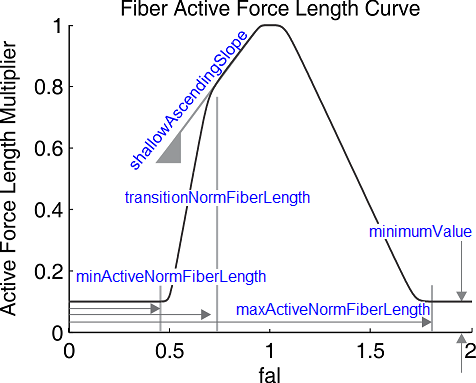
\includegraphics[width=0.5\textwidth,
    keepaspectratio]{active-force-length-curve.png}\label{fig:active-force-length-curve}}
  \subfloat[Passive \gls{fl} curve]{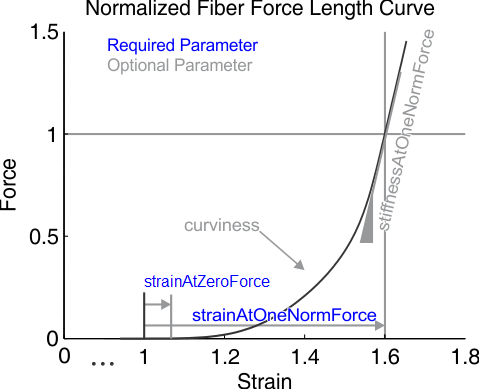
\includegraphics[width=0.5\textwidth,
    keepaspectratio]{passive-force-length-curve.png}\label{fig:passive-force-length-curve}}
  \caption{The active and passive \gls{fl} curve definition of the Millard
    muscle model as implemented in \texttt{OpenSim}.}\label{fig:millard-curves}
\end{figure}

The parameters that describe the above relationships were chosen to fit the
curves found in \hl{Iskander 2018}. In the plots below, we try to match the
\gls{fl} relationships at maximum activation of the lateral rectus muscle. This
represents the first part of testing the fidelity of the model. Due to lack of
data describing the other muscles’ \gls{fl} relationships, we used the
parameters found describing the normalized curves of active and passive \gls{fl}
relationships of the gls{lr} for the other \gls{em} as well.

\gls{em} have a higher fraction of fast twitch fibers and thus different
\gls{fv} behavior, due to different structures compared to skeletal muscles. The
default Millard \gls{fv} curve was used for the six \gls{em}, since the behavior
of the selected muscle model depends mainly on the maximum contraction velocity
$v^{\text{max}}$. The maximum muscle contraction velocity is tuned so as to
match the peak velocity of saccadic eye movement 15.7 rad / s. Following this
definition, the maximum muscle contraction velocity is given in optimal fiber
length per seconds and it is thus different for each \gls{em} since their
optimal fiber length is different. Also, because of different structure of
neural control of eye movements, activation and deactivation delays are lower
than in skeletal muscles, at about 5 ms.

\begin{table}[h]
  \caption{Millard muscle parameters for the
    \gls{em}.}\label{tab:muscle-parameters}
  \begin{tabular}{@{}cccccccccc@{}}
    \toprule
    \thead{Muscle}
    & \thead{Maximum Isometric \\ Force (N)}
    & \thead{Optimal Fiber \\ Length (m)}
    & \thead{Tendon Slack \\ Length (m)}
    & \thead{Maximum Contraction \\ Velocity (m / s)} \\
    \midrule
    \gls{lr} & 1.4710 & 0.04898 & 0.0084 & 3.8483 \\
    \gls{mr} & 1.5740 & 0.04084 & 0.0038 & 4.6155 \\
    \gls{sr} & 1.1768 & 0.04487 & 0.0054 & 4.2009 \\
    \gls{ir} & 1.4269 & 0.04549 & 0.0048 & 4.1437 \\
    \gls{so} & 0.6031 & 0.03956 & 0.0265 & 4.7648 \\
    \gls{io} & 0.5590 & 0.04110 & 0.0015 & 3.5863 \\
    \bottomrule
  \end{tabular}
\end{table}

Wrapping objects help to simulate the proper dynamics. Using wrapping objects
implemented in the \texttt{OpenSim} allows us to model realistic force
directions as the muscle runs over the eyeball. From the point of origin to the
pulley point, the force exerted by the contraction of the muscles is aligned
along one straight line. But, from the pulley point to the insertion point, the
force is distributed along the surface of a sphere. Two separate wrapping
spheres for the rectus muscles and the oblique muscles were created, to avoid
abnormal changes on the \gls{fl} curve as the eyeball rotates in the three
directions.

%%%%%%%%%%%%%%%%%%%%%%%%%%%%%%%%%%%%%%%%%%%%%%%%%%%%%%%%%%%%%%%%%%%%%%%%%%%%%%%% 
\subsection*{Passive Connective Tissues}\label{sec:passive-connective-tissues}

The passive connective tissues of the eyeball apply a restoring force, which
brings the globe back to the central position when the net force from the
\gls{em} is zero. These tissues include all non-muscular suspensory tissues,
such as Tenon’s capsule, the optic nerve, the fat pad and the conjunctiva. The
force-displacement curve of the net elasticity can be represented as

\begin{equation}\label{equ:passive-tissue}
  \vec{f}_t = -k_p \vec{q} - k_c 10^{-3} \vec{q}^3 - k_d * \vec{\dot{q}}
\end{equation}
% 
where, $\vec{f}_t$ represents the passive tissue forces, $k_p= 0.002225$ N m /
rad, $k_c= 34.5297$ N m / (rad^3) and $k_v= 0.002$ N m s / rad the constants and
$\vec{\dot{q}} \inr{3}$ the rotational coordinates of the model. These forces
serve the eye’s stabilization, and are modeled using \texttt{OpenSim}'s
expression based coordinate force.
% 0.33 * 9.8066500286389 * 10**-3 / (numpy.pi / 180) = 0.18542028707494282 * 0.012
% 1.56 * 9.8066500286389 * 10**-3 / (numpy.pi / 180) ** 3 = 2877.4856893811248 * 0.012

%%%%%%%%%%%%%%%%%%%%%%%%%%%%%%%%%%%%%%%%%%%%%%%%%%%%%%%%%%%%%%%%%%%%%%%%%%%%%%%% 
\section*{Results}\label{sec:results}

%%%%%%%%%%%%%%%%%%%%%%%%%%%%%%%%%%%%%%%%%%%%%%%%%%%%%%%%%%%%%%%%%%%%%%%%%%%%%%%% 
\subsection*{Model Validation}\label{sec:model-validation}

To meet good fidelity criteria, a model requires to be verified and
validated. In our study, verification in oculomotor models was performed by
comparing the \gls{fl} characteristic curves of the modeled \gls{em} to
published data. These data include only the lateral rectus characteristic
curves. However, we can make a safe assumption that the other muscles have
similar properties. More characteristic curves showing the \gls{fl} relationship
of the other \gls{em}, as well as the changes in muscle length with rotation in
all directions, are presented in the end of this report. Further verification
can be done by comparing the model’s joint forces produced during horizontal
movement with clinically collected data, but these data are not available.
Validation was performed by simulating and analyzing synthesized eye movements
while ensuring that Listing Law was obeyed by maintaining zero torsion in
secondary gaze positions, and by testing if the assessed innervations are
sufficient in fixating the eye at a desired position.

%%%%%%%%%%%%%%%%%%%%%%%%%%%%%%%%%%%%%%%%%%%%%%%%%%%%%%%%%%%%%%%%%%%%%%%%%%%%%%%% 
\subsection*{Fixation Controller}\label{sec:fixation-controller}

%%%%%%%%%%%%%%%%%%%%%%%%%%%%%%%%%%%%%%%%%%%%%%%%%%%%%%%%%%%%%%%%%%%%%%%%%%%%%%%% 
% \section*{Discussion}\label{sec:discussion}

%%%%%%%%%%%%%%%%%%%%%%%%%%%%%%%%%%%%%%%%%%%%%%%%%%%%%%%%%%%%%%%%%%%%%%%%%%%%%%%% 
\section*{Conclusion}\label{sec:conclusion}

A realistic ocular model that represents the ocular motility of a normal human
eye was presented. The model can be used to simulate different saccadic
movements and obtain the muscle activations required to track the movement. The
model was validated against experimental measured data and is able to synthesize
saccadic movements reasonably well.

We even showed that the simulation results produced by static optimization and
forward dynamics in OpenSim are less satisfactory than the proposed solution
where we used a \gls{pd} controller to minimize the tracking error between the
desired and estimated trajectory of saccadic movements. The desired kinematics
were tracked within a maximum \gls{rmse} of and in horizontal and vertical
saccades respectively. With the application of the controller, a very rapid
instantaneous acceleration and a constant velocity to sustain clear vision is
attained. The produced activation levels were in accordance with the
descriptions found in the bibliography and the highest activation levels were
shown only during the time intervals when the main agonist muscle was activated.

%%%%%%%%%%%%%%%%%%%%%%%%%%%%%%%%%%%%%%%%%%%%%%%%%%%%%%%%%%%%%%%%%%%%%%%%%%%%%%%% 

\bibliography{mylibrary}
\addcontentsline{toc}{chapter}{Bibliography}

%%%%%%%%%%%%%%%%%%%%%%%%%%%%%%%%%%%%%%%%%%%%%%%%%%%%%%%%%%%%%%%%%%%%%%%%%%%%%%%% 
\end{document}

%%% Local Variables:
%%% mode: latex
%%% TeX-master: t
%%% End:
